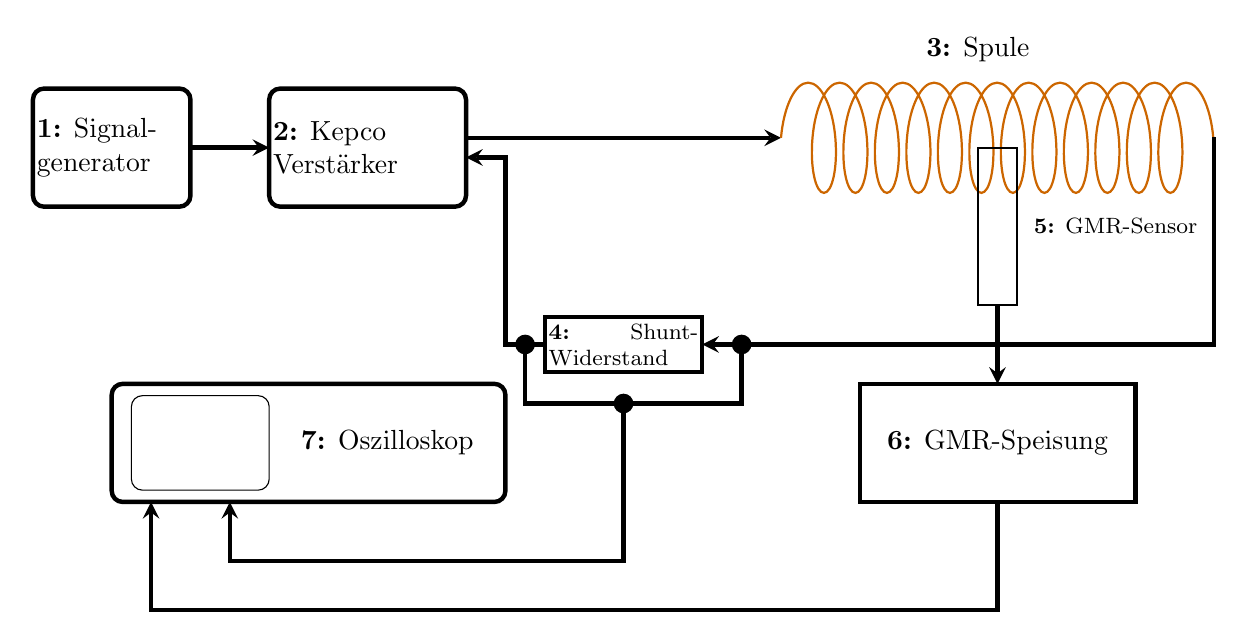
\begin{tikzpicture}[>=stealth]

    % signal generator
    \draw[black,ultra thick,rounded corners] (0,0) rectangle (2,1.5);
    \node at (1,.75) {\parbox{1.9cm}{\textbf{1:} Signal-\\generator}};

    % line from signal generator to amplifier
    \draw[->,ultra thick] (2,.75) -- (3,.75);

    % amplifier
    \draw[black,ultra thick,rounded corners] (3,0) rectangle (5.5,1.5);
    \node at (4,.75) {\parbox{1.9cm}{\textbf{2:} Kepco \\ Verst\"arker}};

    % line from amplifier to coil
    \draw[->,ultra thick] (5.5,.75+.125) -- (9.5,.75+.125);

    % coil
    \draw[thick,color=orange!80!black,decoration={aspect=0.35, segment length=4mm, amplitude=7mm,coil},decorate] (9.5,.75+.125) -- (15,.75+.125);
    \node at (12,2) {\textbf{3:} Spule};

    % line from right side of coil to shunt resistor
    \draw[->,ultra thick] (15,.76+.125) -- (15,-1.75) -- (8.5,-1.75);

    % shunt resistor
    \draw[black,ultra thick] (6.5,-1.75+.7/2) rectangle (8.5,-1.75-.7/2);
    \node at (7.5,-1.75) {\footnotesize\parbox{1.9cm}{\textbf{4:} Shunt-Widerstand}};

    % line from shunt resistor to amplifier
    \draw[->,ultra thick] (6.5,-1.75) -- (6,-1.75) -- (6,.75-.125) -- (5.5,.75-.125);

    % GMR sensor
    \draw[black,thick] (12,0.75) rectangle (12.5,-1.25);
    \node at (13.75,-0.25) {\footnotesize{\textbf{5:} GMR-Sensor}};

    % line from GMR sensor to GMR box
    \draw[->,ultra thick] (12.25,.-1.25) -- (12.25,-2.25);

    % GMR box
    \draw[black,ultra thick] (14,-2.25) rectangle (10.5,-3.75);
    \node at (12.25,-3) {\textbf{6:} GMR-Speisung};

    % line from GMR box to oscilloscope
    \draw[->,ultra thick] (12.25,-3.75) -- (12.25,-5-.125) -- (1.5,-5-.125) -- (1.5,-3.75);

    % oscilloscpe
    \draw[black,ultra thick,rounded corners] (6,-2.25) rectangle (1,-3.75);
    \draw[black,rounded corners] (3,-2.4) rectangle (1.25,-3.6);
    \node at (4.5,-3) {\textbf{7:} Oszilloskop};

    % Measurement of shunt voltage
    \draw[-,ultra thick] (6.25,-1.75) -- (6.25,-2.5) -- (7.5-.125,-2.5);
    \draw[-,ultra thick] (9,-1.75) -- (9,-2.5) -- (7.5+.125,-2.5);
    \fill (7.5,-2.5) circle [radius=0.125];
    \draw[->,ultra thick] (7.5,-2.5) -- (7.5,-4.5)  -- (2.5,-4.5) -- (2.5,-3.75);
    \draw[-,ultra thick] (6.25 - 0.025,-2.5) -- (8.75 + 0.025,-2.5);
    \fill (6.25,-1.75) circle [radius=0.125];
    \fill (9,-1.75) circle [radius=0.125];
\end{tikzpicture}
